\documentclass[english,xcolor=x11names]{beamer}
\usepackage[utf8]{inputenc}
\usepackage[T1]{fontenc}
\usepackage{babel}
\usepackage{graphicx}
\usepackage{tikz}
\usepackage{pgfplots}
\usepackage{hyperref}
\usepackage{libertine}
\usepackage{eulervm}
\usepackage[ttdefault]{sourcecodepro}
\usepackage{fontawesome5} 
\usepackage{relsize}
\usepackage{amsmath}
\usepackage{amssymb}
\usepackage{bm}
\usepackage[autostyle=true]{csquotes} 
\usepackage[backend=biber,style=authoryear,citestyle=alphabetic,maxnames=1,url=false,doi=false,isbn=false,dashed=false,mincrossrefs=1000]{biblatex}
\usepackage{apptools}
\usepackage{appendixnumberbeamer}
\usepackage{tikz}
\usepackage{listings}
\usepackage{xspace}
\usepackage{biblatex}
\usepackage{tabularx}
\usepackage{booktabs}
\usepackage{graphicx}

\let\tmp\mod \let\mod\bmod \let\bmod\tmp
\let\varemptyset\emptyset \let\emptyset\varnothing
\let\tmp\epsilon \let\epsilon\varepsilon \let\varepsilon\tmp
\let\tmp\phi \let\phi\varphi \let\varphi\tmp

\usetheme{boxes} % Simple
\definecolor{mlugreen}{RGB}{0,81,51}
\setbeamercolor{structure}{fg=mlugreen}
\usefonttheme[onlymath]{serif}
\setbeamerfont{title}{series=\bfseries,parent=structure}
\setbeamersize{description width=2em}
\setbeamersize{text margin left=0.5cm, text margin right=0.5cm}
\setbeamercovered{transparent}
\setbeamertemplate{frametitle continuation}[from second][\usebeamercolor{normal text}\color{fg!40!bg}\insertcontinuationtext] 
\beamertemplatenavigationsymbolsempty
\addtobeamertemplate{navigation symbols}{}{%
	\usebeamerfont{footline}%
	\usebeamercolor[fg]{footline}%
	\quad%
	\raisebox{0.5ex}{\IfAppendix{A-}{}\insertframenumber/\inserttotalframenumber}%
	\enskip%
	\vspace{0.5ex}%
}
\defbeamertemplate{description item}{align left}{\insertdescriptionitem\hfill}
\setbeamertemplate{description item}[align left]

\newcommand{\textttsmall}[1]{\texttt{\smaller #1}}
\newcommand{\query}[1]{\textttsmall{#1}}
\newcommand{\domain}[1]{\href{http://#1}{\mbox{\textttsmall{#1}}}}

\renewcommand{\bibfont}{\smaller}
\renewcommand{\pgfuseimage}[1]{\includegraphics[scale=.65]{#1}} % Shrink book images.
\setlength{\bibhang}{0pt} % Remove hanging indent.
\AtEveryCite{\smaller\color{fg!60!bg}} % Make cites smaller, dimmed.

\pgfplotsset{
  compat=1.18
}
\definecolor{mediumgray}{gray}{0.60}
\definecolor{webiscodebasic}{rgb}{0.2,0.2,0.2}
\definecolor{webiscodekeyword}{rgb}{0.0,0.5,0.0}
\definecolor{webiscodekeywordself}{rgb}{0.7,0.4,0.6}
\definecolor{webiscodeidentifier}{rgb}{0.0,0.0,0.0}
\definecolor{webiscodecomment}{rgb}{0.25,0.5,0.5}
\definecolor{webiscodestring}{rgb}{0.75,0.12,0.12}
\definecolor{webiscodedecorator}{rgb}{0.6,0.3,0.0}
\lstdefinestyle{webisstyle}{
  basicstyle=\fontsize{6pt}{7pt}\selectfont\ttfamily\color{webiscodebasic},
  keywordstyle=\color{webiscodekeyword},
  identifierstyle=\color{webiscodeidentifier},
  commentstyle=\color{webiscodecomment},
  stringstyle=\color{webiscodestring},
  showstringspaces=false,
  frame=lines,
  framesep=0.7em,
  rulesep=0.5em,
  framerule=0.1em,
  keepspaces=true,
  tabsize=2,
  showtabs=false,
  numbers=none,
  literate=
    {->}{{\textrightarrow}}{2}
    {>=}{{\(\geq\)}}{2}
    {<=}{{\(\leq\)}}{2}
    {!=}{{\(\neq\)}}{2},
}
\lstloadlanguages{Python}
\lstset{
  style=webisstyle,
  language=Python,
  emph={[1]def,class},
  emphstyle={[1]\color{webiscodekeyword}\bfseries},
  emph={[2]self,cls},
  emphstyle={[2]\color{webiscodekeywordself}},
  emph={[3]@dataclass},
  emphstyle={[3]\color{webiscodedecorator}},
}

\newcommand{\bibliographyframe}{
\begin{frame}[t,allowframebreaks]{References}
	\begin{thebibliography}{10}
		\beamertemplatebookbibitems
		\printbibliography
	\end{thebibliography}
\end{frame}
}
\newcommand{\titleframe}{
	\begingroup
	\setbeamertemplate{navigation symbols}{}
	\frame[plain]{\titlepage}
	\endgroup
}

\newcommand{\pro}{\item[\(\bm{+}\)]} % Pro item
\newcommand{\contra}{\item[\(\bm{-}\)]} % Contra item
\newcommand{\thankyouname}{Thank you, stay tuned for more!}
\newcommand{\thankyou}{\vfill\hfill\emph{\thankyouname}}
\newcommand{\todocite}{{\smaller\color{red}[CITE]}\xspace}
\newcommand{\todo}[1]{{\smaller\color{red}[#1]}}

% Bibliography
% \addbibresource{TODO.bib}

\title{\faIcon{greater-than-equal}~\textbf{\texttt{ir\_axioms}}}
\subtitle{Intuitive Axiomatic Retrieval Experimentation.\vspace*{-0.5cm}}
\author{\scriptsize A.~Bondarenko \and M.~Fröbe \and J.~H.~Reimer \and B.~Stein \and M.~Völske \and M.~Hagen}
\institute{}
\date{}
\titlegraphic{\vspace*{-1.5cm}
\includegraphics[width=4cm]{meme-ranking.jpg}
}

\begin{document}

\titleframe

\begin{frame}{Axioms}
  \framesubtitle{What they promise~\faIcon{grin-wink}}
  \begin{columns}
    \begin{column}{0.6\textwidth}
      \begin{itemize}
        \item Axioms are (pairwise) \textbf{preferences}
        \item[\(\bm{\approx}\)] \textquote{Rules} what documents to rank first
        \item \textbf{Easy} to understand
      \end{itemize}
      \begin{block}{Use-cases}
        \begin{itemize}
          \item Explain ranker decisions
          \item Evaluate ranking errors
          \item Re-rank
        \end{itemize}
      \end{block}
    \end{column}
    \begin{column}{0.4\textwidth}
      \begin{center}
        
\includegraphics[width=4cm]{meme-great-idea.jpg}
      \end{center}
    \end{column}
  \end{columns}
\end{frame}

\begin{frame}{Working with axioms\textellipsis~\faIcon{meh}}
  \framesubtitle{in the past}
  \begin{columns}
    \begin{column}{0.6\textwidth}
      \begin{center}
        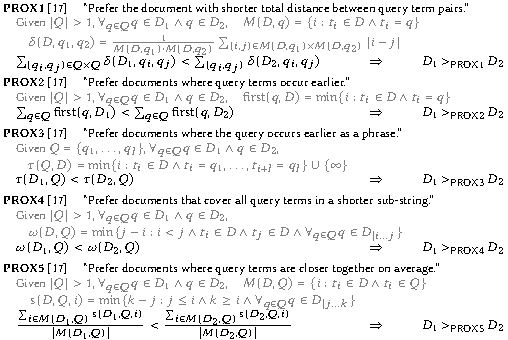
\includegraphics[width=4.75cm]{axiom-definitions.pdf}
      \end{center}
      \begin{block}{Problems}
        \begin{itemize}
          \item Not always \textquote{easy to understand}\,\texttt{\texttrademark}
          \item Many implementation caveats~(uff!)
          \color{fg!60!bg}
          \item Hard to maintain etc.\textellipsis
        \end{itemize}
      \end{block}
    \end{column}
    \begin{column}{0.4\textwidth}
      \begin{center}
        
\includegraphics[width=4cm]{meme-whoa-easy.jpg}
      \end{center}
    \end{column}
  \end{columns}
\end{frame}

\begin{frame}{\textbf{\texttt{ir\_axioms}} to the rescue!}
  \framesubtitle{%
    \scriptsize%
    \href{https://github.com/webis-de/ir_axioms}{\faIcon{github}\enskip\texttt{webis-de/ir\_axioms}}
    \quad
    \href{https://pypi.org/project/ir_axioms/}{\faIcon{python}\enskip\texttt{pip install ir\_axioms}}
  }
  \begin{itemize}
    \item Reference implementations for \textbf{25~common axioms}
    \item \textbf{Define and combine} axioms declaratively
    \item Tightly integrates with \textbf{PyTerrier \& Pyserini}
  \end{itemize}
  \begin{columns}[t]
    \begin{column}{0.5\textwidth}
      \begin{block}{Experiments}
        \lstinputlisting[firstline=2]{listing-pyterrier-experiment.py}
      \end{block}
    \end{column}
    \begin{column}{0.5\textwidth}
      \begin{block}{Re-ranking}
        \lstinputlisting[firstline=2]{listing-pyterrier-reranking.py}
      \end{block}
    \end{column}
  \end{columns}
  \thankyou
\end{frame}

% \appendix
% \bibliographyframe

\end{document}